\documentclass[11pt,a4paper]{article}
\usepackage[T1]{fontenc}
\usepackage[utf8]{inputenc}
\usepackage{lmodern,amsmath,amssymb,booktabs,tabularx,array,graphicx,microtype}
\usepackage[a4paper,margin=25mm]{geometry}
\usepackage{xcolor}
\usepackage[colorlinks=true,linkcolor=blue!45!black,urlcolor=blue!45!black,citecolor=blue!45!black]{hyperref}
\usepackage{placeins}
\raggedbottom
\setcounter{topnumber}{3}
\renewcommand{\topfraction}{.88}
\renewcommand{\textfraction}{.10}
\hypersetup{pdftitle={Programación de vertidas y control térmico de una fundación de hormigón masivo bajo incertidumbre},pdfauthor={Grupo 2 · MCOC},pdflang={es-CL}}
\renewcommand{\figurename}{Figura}
\renewcommand{\tablename}{Tabla}
\renewcommand{\refname}{Referencias}
\newcommand{\plan}[1]{\texttt{#1}}
\newcommand{\unit}[1]{\,\mathrm{#1}}
\newcommand{\dd}{\,\mathrm{d}}
\setlength{\emergencystretch}{2em}
\setlength{\parskip}{.4em}
\setlength{\parindent}{0pt}
\title{Programación de vertidas y control térmico de una fundación de hormigón masivo bajo incertidumbre}
\author{Grupo 2\\Métodos Computacionales en Obras Civiles · Proyecto 2\\Universidad de los Andes, Chile}
\date{23 de noviembre de 2026}
\begin{document}
\maketitle
\begin{center}\textbf{Resumen}\end{center}
Se estudia la colocación de una fundación de aerogenerador en Freirina, Chile, con el objetivo de minimizar su duración y mantener la probabilidad conjunta de exceder 70 °C o un diferencial de 20 °C en no más de 5\%. Se discretizó una geometría IFC de 636,878 m³ mediante volúmenes finitos con activación por vertida. Ocho fuentes de hidratación inferidas en probetas y tres miembros representativos de un pronóstico GFS definieron 24 escenarios ponderados por plan. Se compararon nueve programas mediante enumeración, tomando el diferencial entre el máximo del hormigón activo y el mínimo a profundidad nominal de 25 mm en el mismo instante. Ocho alternativas registraron entre 85\% y 100\% de falla. El programa experimental \plan{moderate\_20}, con colocación en cinco vertidas, refrigeración por agua y retiro gradual de aislamiento, terminó la colocación a las 14,738 h y produjo cero excedencias en 744 h de evaluación. Los máximos nominales fueron 49,599 °C y 19,158 °C. El peor control espacial elevó el diferencial a 19,621 °C. El cumplimiento es condicional al modelo discreto. La representación de superficies, los pesos hipotéticos y la factibilidad de suministro y refrigeración limitan su extrapolación a obra.

\textbf{Palabras clave.} Hormigón masivo, hidratación, volúmenes finitos, refrigeración interna, confiabilidad térmica.

\section{Introducción}
La hidratación del cemento libera calor en el volumen del hormigón. En una fundación gruesa, la disipación por unidad de volumen disminuye al aumentar la distancia entre el núcleo y los bordes. El interior conserva parte de la energía mientras la superficie responde al ambiente, al terreno y a las protecciones temporales. La dilatación durante el calentamiento y la contracción durante el enfriamiento pueden generar tensiones bajo restricción. El desarrollo de rigidez, la fluencia, la evolución resistente y la restricción externa intervienen en el paso de un campo térmico a una fisura \cite{aci,ciria}. Este estudio calcula temperaturas y excedencias térmicas. Un pronóstico mecánico requeriría una ley constitutiva dependiente de la edad y datos adicionales sobre restricción, resistencia y deformación.

Programar vertidas más juntas acorta el tiempo de bombeo con esperas, pero superpone el calor de capas que todavía se hidratan. Aumentar las esperas expone temporalmente las interfaces y cambia el intercambio con el ambiente. El aislamiento modera el descenso superficial y puede retener calor en el núcleo. Retirarlo abre una vía de disipación al mismo tiempo que puede intensificar el diferencial. Una tubería interior ofrece una segunda vía, cuyo efecto depende de la temperatura y capacidad térmica del agua, del contacto con el hormigón y de su operación en el tiempo. La decisión requiere examinar conjuntamente esos mecanismos y distinguir la duración de colocación del tiempo de curado.

La pregunta es qué programa termina primero entre las alternativas evaluadas y satisface el requisito probabilístico. Los valores de 70 °C para temperatura máxima, 20 °C para diferencial y 5\% para excedencia conjunta se adoptan como criterios docentes \cite{e14}; la bibliografía da contexto físico y metodológico. Se aplica la misma distribución de escenarios a todas las alternativas y se contrastan las dos formulaciones de riesgo disponibles, la enumeración de un soporte finito y el muestreo de ese soporte. Se mantiene la trazabilidad entre la formulación publicada en E14, la recomendación provisional de E15 y la evidencia de refrigeración conservada para F02 \cite{e14,e15,f02}. Se considera decisiva la diferencia entre satisfacer el criterio en esa matriz y disponer de evidencia suficiente para autorizar el uso en terreno.

\section{Caso de estudio y datos}
\subsection*{Geometría, emplazamiento y colocación}
El emplazamiento de referencia corresponde al entorno del Parque Eólico Sarco, comuna de Freirina, Región de Atacama. La consulta nominal para las condiciones de borde fue 28,856102° S, 71,421831° O. El proveedor devolvió el nodo 29,0° S, 71,5° O y una elevación informada de 145 m. Esas coordenadas documentan la solicitud y la celda meteorológica. La identificación geodésica fina de cada fundación y una serie local de contraste quedan pendientes.

El IFC aporta cinco sólidos secuenciales. Su caja envolvente mide 18 × 18 × 4,30 m. Los niveles de separación se sitúan a 0,55, 1,10, 2,20 y 3,30 m sobre la base. La cuarta y quinta vertidas ocupan anchos máximos aproximados de 12,50 y 7,00 m, respectivamente. La discretización clasifica centros de una retícula cartesiana contra esos sólidos y asigna a cada centro ocupado una etiqueta de vertida. En la malla nominal se obtienen 28\,652 celdas de $0{,}45\times0{,}45\times0{,}11$ m, con 638,2233 m³ frente a 636,8777 m³ del IFC y 636,8850 m³ de la referencia analítica de E14. El error volumétrico firmado es aproximadamente +0,211\%. Las capas representan, en orden ascendente, 147,626, 147,626, 214,224, 88,925 y 38,477 m³ según el calendario a 50 m³/h. El perímetro curvo se convierte en caras ortogonales y la elevación de las interfaces se aproxima con planos discretos. La Figura~\ref{fig:ifc} muestra esta partición y su representación. Se conserva la misma fundación final al activar las cinco etiquetas individualmente o simultáneamente.

\begin{figure}[htbp]
\centering
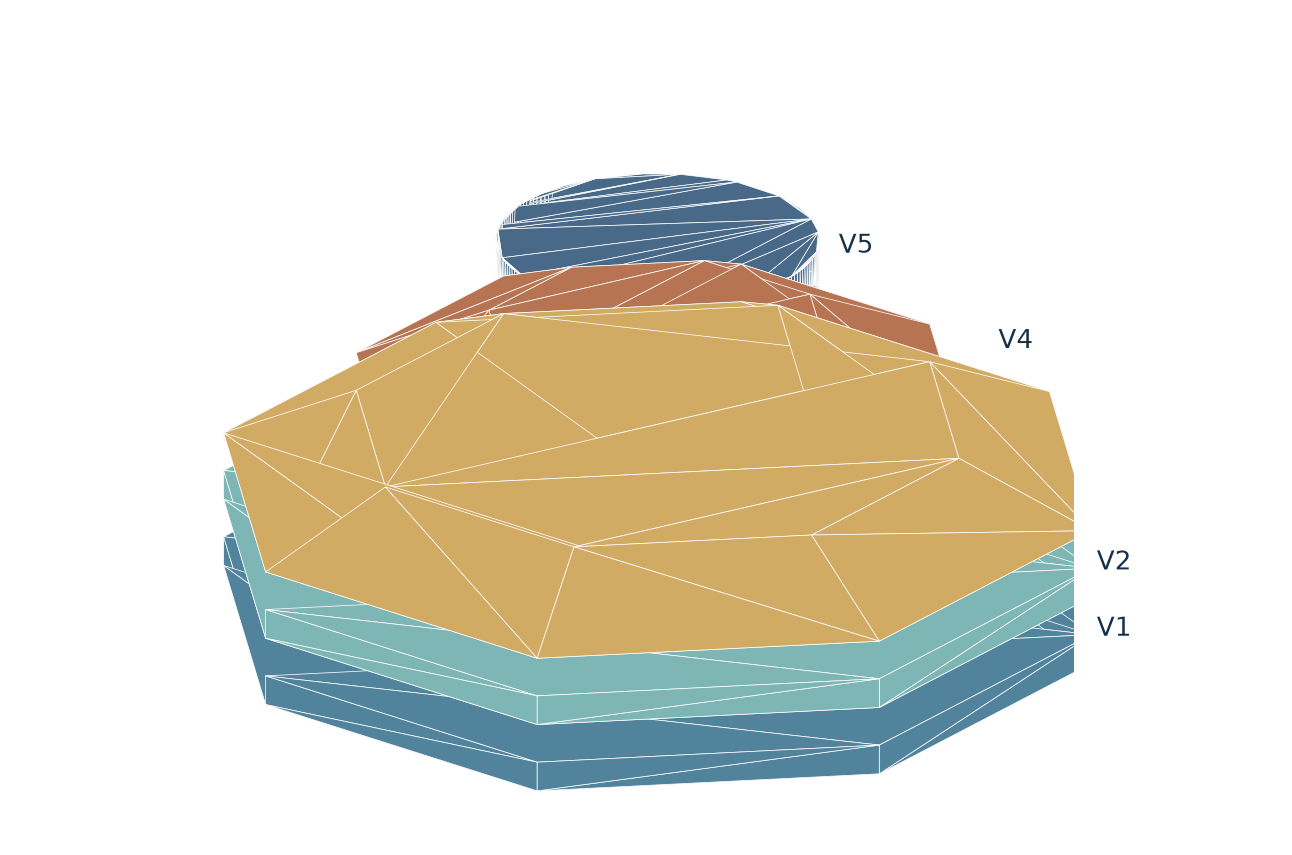
\includegraphics[width=.75\linewidth]{figuras/ifc_stages.png}
\caption{Partición de la fundación IFC por vertidas. Coordenadas locales en metros. Evidencia geométrica E14/F02.}
\label{fig:ifc}
\end{figure}

\begin{table}[htbp]
\centering\small
\caption{Parámetros de la configuración nominal \plan{moderate\_20}. Los parámetros de diseño se deben comprobar en obra.}
\label{tab:param}
\begin{tabularx}{\linewidth}{@{}lXlll@{}}
\toprule
Símbolo & Magnitud & Unidad & Valor & Fuente y clase \\
\midrule
$V$ & Volumen final IFC & m³ & 636,8777 & IFC, cálculo \\
$\rho$ & Densidad en fundación & kg/m³ & 2400 & E08/F02, supuesto \\
$c_p$ & Calor específico en fundación & J/(kg K) & 900 & E08/F02, supuesto \\
$k$ & Conductividad en fundación & W/(m K) & 2 & E08/F02, supuesto \\
$T_{0,j}$ & Temperatura de colocación & °C & 5 & F02, supuesto \\
$r$ & Ritmo de colocación & m³/h & 50 & F02, supuesto \\
$h_a$ & Película exterior & W/(m² K) & 8 & E14/F02, supuesto \\
$T_g$ & Reservorio del suelo & °C & 18 & E14/F02, supuesto \\
$k_g,\ell_g$ & Conductividad y profundidad suelo & W/(m K), m & 1,5 y 0,40 & E14/F02, supuesto \\
$T_{w,\mathrm{ent}}$ & Entrada de agua & °C & 20 & F02, supuesto \\
$\dot V_w$ & Caudal por ramal & L/s & 0,25 & F02, supuesto \\
$\ell_\Sigma$ & Longitud activa total & m & 198,62 & F02, cálculo \\
$D_i,D_o$ & Diámetros interior y exterior & mm & 26 y 32 & F02, diseño \\
$k_p$ & Conductividad de pared del tubo & W/(m K) & 0,40 & F02, supuesto \\
$d$ & Profundidad nominal S25 & mm & 25 & Criterio docente \\
\bottomrule
\end{tabularx}
\end{table}

\subsection*{Hidratación}
El archivo archivado \plan{source\_terms.txt} contiene tasas volumétricas ya inferidas para ocho probetas cilíndricas de radio 37,5 mm y altura 150 mm. Su cabecera informa $\rho=2476$ kg/m³, $c_p=1023$ J/(kg K) y dosificación de cemento de 350,77 kg/m³ para el diseño atribuido a Arrieta. La inversión reportada usa volúmenes finitos axisimétricos, 16 bases B-spline cúbicas, corrección de offsets por sensor y penalización de segundas diferencias de 0,05. La conductancia superficial nominal usada en esa inversión es 2,5 W/(m² K). Se ensayan valores de 2,1 y 3,0 W/(m² K) en la cabecera, lo que cambia materialmente la energía inferida. Por ejemplo, M4 SS pasa de 84,3 a 120,1 MJ/m³ a lo largo de ese intervalo. Esa dependencia de la inversión justifica tratar la energía como una fuente de incertidumbre.

La campaña SS se identifica como 13--20 de abril de 2025 y 22A como 22 de abril de 2025. En SS la cabecera reporta errores de ajuste del orden de 0,1--0,2 K y en 22A del orden de 0,4 K. El sensor ambiental único de 22A explica peor el ciclo observado. Se usa el tiempo tabulado desde el comienzo de la ventana retenida, dos horas después del comienzo del registro. La discretización nominal de las series es de 10 min. Se conservan los pares finitos ordenados y se interpreta el tramo \texttt{NaN} de 22A como ausencia de registros. Las edades en horas se convierten a segundos antes de integrar. El insumo es potencia por metro cúbico. Su producto por tiempo y volumen entrega energía en julios. Multiplicar además por la dosificación de cemento contaría dos veces la conversión volumétrica.

La Tabla~\ref{tab:hid} integra cada registro finito por trapecios. El solver interpola la tasa linealmente y usa un potencial integrado para combinar edades y pasos. Cuando termina la curva tabulada se aplica la política exponencial de 24 h de E14; si la tasa terminal es cero, esa extensión aporta cero energía. En M1 SS el aporte eleva el valor de 88,148 a 88,284 MJ/m³ aproximadamente. Se conserva cada curva completa de la biblioteca en su propio escenario. El inicio térmico por vertida es una alineación de la ventana retenida con la edad computacional. Las temperaturas sin procesar, el protocolo completo de mezcla y la fase de ensayo de las primeras dos horas no están documentados en la evidencia usada. Por ello la energía integrada caracteriza la fuente tabulada y sus hipótesis de extensión.

\begin{table}[htbp]
\centering\small
\caption{Ocho fuentes volumétricas. Energía del tramo finito calculada sobre el archivo publicado. Peso de material concordante con E14.}
\label{tab:hid}
\begin{tabular}{@{}lrrrr@{}}
\toprule
Curva & Última edad (h) & Pico (W/m³) & Integral (MJ/m³) & Peso \\
\midrule
M1 SS  &240,333&467,75&88,148&0,20\\
M2 SS  &240,333&531,11&95,715&0,20\\
M3 SS  &240,333&553,01&94,149&0,20\\
M4 SS  &240,333&568,94&100,166&0,20\\
M1 22A &163,000&473,38&61,212&0,05\\
M2 22A &163,000&625,29&82,446&0,05\\
M3 22A &163,000&589,70&73,289&0,05\\
M4 22A &163,000&596,08&73,628&0,05\\
\bottomrule
\end{tabular}
\end{table}

\subsection*{Meteorología}
Open-Meteo archivó la respuesta del ensemble de pronóstico GFS 0,5° solicitada el 17 de noviembre de 2026 a las 18:42:24 UTC, 15:42:24 en Chile continental \cite{openmeteo,e14}. El registro identifica el modelo solicitado como \plan{gfs05} y deja sin valor la corrida y versión interna del proveedor. La respuesta incluye temperatura a 2 m, viento a 10 m y radiación de onda corta. La operación usa sólo temperatura exterior en el borde nominal. El archivo ya tiene cadencia horaria interpolada por la API a partir de la resolución temporal del producto. La reducción minimiza la suma de distancias cuadráticas entre historias de temperatura durante 600 h comunes. De 31 miembros tratados inicialmente como equiprobables, los medoides 0, 13 y 17 representan grupos de 15, 12 y 4 miembros, respectivamente. La distorsión archivada es 0,974 °C² y la máxima distancia RMS al representante es 1,354 °C.

Se seleccionan miembros enteros. Así se retiene el orden de los ciclos diurnos y la persistencia de cada historia, y cualquier variable archivada adicional sigue asociada a su miembro. Los casos de 744 h usan la extensión disponible de esos mismos miembros hasta el 20 de diciembre a las 11:00 UTC. El soporte es una reducción de un pronóstico específico. La dispersión reducida no representa por sí sola sesgos mesoescalares, olas anómalas ni clima de otras fechas. La Figura~\ref{fig:inputs} compara las historias y las tasas que gobiernan la entrada energética.

\begin{figure}[htbp]
\centering
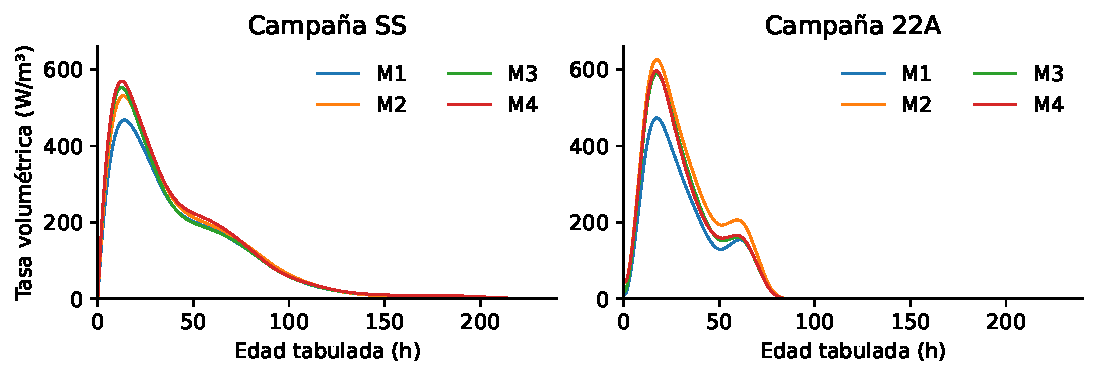
\includegraphics[width=.78\linewidth]{figuras/hidratacion.pdf}\par
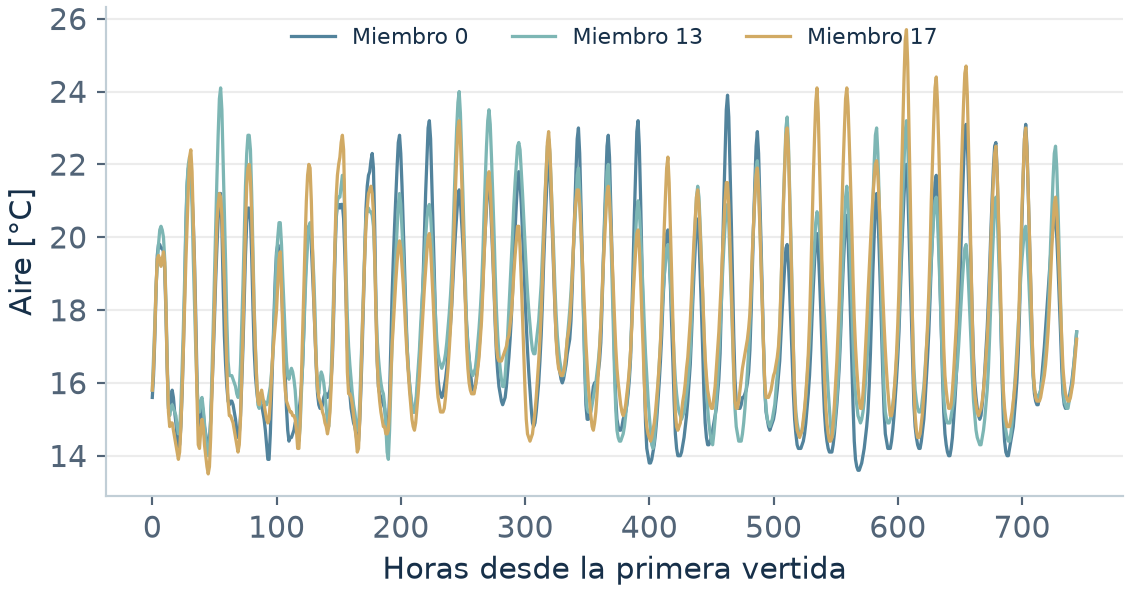
\includegraphics[width=.70\linewidth]{figuras/weather.png}
\caption{Tasas de hidratación archivadas e historias meteorológicas representativas. Eje temporal de hidratación en edad de vertida, eje meteorológico relativo al inicio común.}
\label{fig:inputs}
\end{figure}

\section{Modelo continuo}
Sea $\Omega_j$ el sólido de la vertida $j$ y $t_j$ su instante de inicio. El dominio activo es $\Omega_c(t)=\bigcup_{j:t\ge t_j}\Omega_j$. Cada volumen nuevo entra a temperatura uniforme $T_{0,j}$ y su fuente depende de la edad $a_j=t-t_j$. Antes de la activación no tiene capacidad, flujo interior ni término de hidratación en el problema discreto. La colocación consume tiempo en el cronograma, pero activar al comienzo atribuye capacidad y calor a todo el volumen de la etapa desde ese instante. Este desacople puede importar en las vertidas de más de cuatro horas y, en particular, en la comparación con una sola vertida de 12,738 h.

Con densidad $\rho$ en kg/m³ y capacidad específica $c_p$ en J/(kg K), la variación energética en un subvolumen fijo $B$ de hormigón ya activo se iguala a la potencia entrante más la generación local. La ley de Fourier relaciona el vector flujo $\mathbf q$ en W/m² con el gradiente mediante $\mathbf q=-k\nabla T$, donde $k$ se mide en W/(m K). Por el teorema de la divergencia y localización del balance,
\begin{align}
\frac{\dd}{\dd t}\int_B \rho c_p(T-T_*)\dd V
  &= -\int_{\partial B}\mathbf q\cdot\mathbf n\dd A
     +\int_B \dot q_{h,m}(a_j)\dd V-\dot Q_{w,B},\label{eq:inte}\\
\rho c_p\partial_t T &= \nabla\cdot(k\nabla T)+\dot q_{h,m}(a_j)
\qquad \text{fuera del intercambio con tubos}.\label{eq:pde}
\end{align}
Aquí $T_*$ es una referencia fija arbitraria, $m$ una curva de material, $\dot q_{h,m}$ la fuente en W/m³ y $\dot Q_{w,B}$ la transferencia neta hacia el agua en W. El código localiza esta última transferencia en las celdas recorridas por cada segmento. Una fuente adiabática en forma de aumento de temperatura requeriría $\dot q_h=\rho c_p\dd(\Delta T_{ad})/\dd a$. Una curva acumulada por masa de cemento requeriría multiplicar su derivada temporal por kg de cemento por m³. La entrada de este estudio ya está en W/m³ y se usa directamente.

Se aproxima un medio homogéneo de propiedades constantes. En la unión de dos vertidas activas se conserva el flujo y se adopta continuidad térmica de contacto perfecto. Las caras que miran a una vertida futura se consideran expuestas hasta la activación vecina. Al activarse ésta se elimina el intercambio exterior en la cara compartida y se impone conducción interna. La Tabla~\ref{tab:bordes} resume los cierres. Los parámetros para el aire llevan una película equivalente y las capas sólo agregan resistencia. El suelo es un reservorio con resistencia en serie. Se omiten almacenamiento térmico explícito en moldaje y terreno, lluvia, evaporación, radiación, viento variable y cinética de hidratación dependiente de temperatura. Estas omisiones limitan la transferencia del resultado al curado real, especialmente al suponer colocación a 5 °C.

\begin{table}[htbp]
\centering\small
\caption{Condiciones térmicas por superficie y etapa para F02. $q_n$ es flujo saliente en W/m²; parámetros de E14 y configuración del plan F02.}
\label{tab:bordes}
\begin{tabularx}{\linewidth}{@{}lX X@{}}
\toprule
Superficie & Cierre & Etapa y parámetros \\
\midrule
Lateral y superior & $q_n=(T_f-T_a)/(h_a^{-1}+\sum b_l/k_l)$ & Tablero 18 mm, $k=0{,}13$ W/(m K); aislante $k=0{,}04$, de 100 a 50 mm en h 360 y a 25 mm en h 528. \\
Tras retiro & $q_n=h_a(T_f-T_a)$ & Desde h 672. $h_a=8$ W/(m² K). \\
Base en terreno & $q_n=(T_f-T_g)/(R_c+\ell_g/k_g)$ & Siempre que esté activa. $R_c=0{,}025$ m² K/W. \\
Frente temporal & Cierre exterior de su orientación mientras la vecina está inactiva & Se extingue al activarse la vertida vecina. \\
Interfaz interna & Continuidad térmica y de flujo & Contacto perfecto entre dos lados activos. \\
\bottomrule
\end{tabularx}
\end{table}

\subsection*{Intercambio con el agua}
\plan{moderate\_20} distribuye 29 ramales en las vertidas 3 a 5, en cotas de 1,42, 1,91, 2,48, 3,01 y 3,83 m. El trazado nominal usa radio de 5 m, espaciamiento transversal de 1,6 m y margen geométrico de 0,18 m. Se estima además unos 119 m de conexión al moldaje aislada térmicamente, con colectores por diseñar. En un segmento de longitud $\ell$, la resistencia lineal $R'$ en K m/W suma película interior, pared y conducción radial equivalente en el hormigón,
\begin{equation}
R'=\frac{1}{h_w\pi D_i}+\frac{\ln(D_o/D_i)}{2\pi k_p}
  +\frac{\ln(r_e/(D_o/2))}{2\pi k},\quad
r_e=\sqrt{\Delta y\Delta z/\pi},\quad UA=\ell/R'.
\label{eq:resist}
\end{equation}
En la malla nominal $R'=0{,}2521$ K m/W. $h_w$ proviene de la correlación de Gnielinski en flujo interno turbulento \cite{gnielinski}. Se usan las propiedades constantes del agua publicadas con el kernel y el caudal por ramal de 0,25 L/s. En flujo pistón cuasiestacionario, con $T_i$ representativa de la celda y $\dot m_w c_w$ en W/K, el avance en el segmento es
\begin{equation}
T_{w,o}=T_i+(T_{w,e}-T_i)e^{-UA/(\dot m_w c_w)},
\qquad \dot Q_{w,i}=\dot m_w c_w(T_{w,o}-T_{w,e}).
\label{eq:water}
\end{equation}
La ecuación~\eqref{eq:water} integra $\dot m_w c_w\,\dd T_w/\dd x=(T_i-T_w)/R'$ desde la entrada, con $T_i$ uniforme por segmento. Con $\rho_w=998$ kg/m³, $c_w=4182$ J/(kg K), $\mu_w=1{,}002$ mPa s y $k_w=0{,}598$ W/(m K) del kernel, se obtiene $v=0{,}471$ m/s, $Re\approx 12\,194$, $Pr\approx 7{,}01$ y $h_w\approx 2194$ W/(m² K). Son estimaciones para los ramales rectos bajo las hipótesis del modelo. La Figura~\ref{fig:ramales} muestra el trazado activo archivado.

\begin{figure}[htbp]
\centering
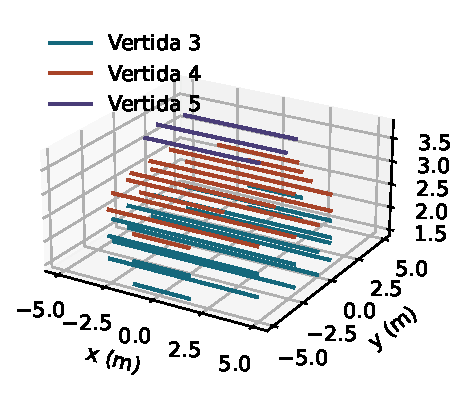
\includegraphics[width=.68\linewidth]{figuras/ramales.pdf}
\caption{Ramales activos del diseño nominal. Los segmentos se dibujan a partir de las coordenadas archivadas. Conexiones exteriores, armadura y colectores requieren diseño de obra.}
\label{fig:ramales}
\end{figure}

La salida se propaga como entrada del segmento siguiente y el calor ganado por el agua se resta en la celda sede. Se desvía un ramal completo si su balance neto calentaría al sólido, aunque pueden existir tramos individuales que cedan calor. Se impuso un máximo de 35 kW y una ventana de h 18 a 552. El máximo combinado de caudal es 7,25 L/s. El control fino reportó demanda de hasta 12,00 kW y extracción acumulada de hasta 12,534 GJ. La comparación no activa el máximo de potencia como mecanismo dominante. Las exigencias hidráulicas reales incluyen pérdidas en colectores y accesorios, disponibilidad de agua y capacidad de mantener el régimen térmico. La correlación y la resistencia equivalente no resuelven el gradiente inmediato en la vecindad física del tubo.

\section{Discretización y algoritmos}
Para la celda $i$ de volumen $V_i$, $C_i=\rho_i c_{p,i} V_i$ es la capacidad en J/K. Al integrar la ecuación~\eqref{eq:pde} por celda y usar la cara compartida de área $A_{ij}$ se obtiene
\begin{align}
 C_i\frac{\dd T_i}{\dd t}
 &=\sum_{j\in\mathcal N_i}G_{ij}(T_j-T_i)
   -\sum_b A_b q_b + V_i\dot q_{h,m}(a_i)-\dot Q_{w,i},\\
 G_{ij}&=\frac{A_{ij}}{d_i/k_i+d_j/k_j}.
\end{align}
$d_i$ y $d_j$ son distancias de centro a cara. El flujo simétrico cancela en la suma energética entre dos celdas. Para ambiente y suelo, la conducción de media celda se suma a la resistencia exterior $R_b$ de la Tabla~\ref{tab:bordes}. Así, $q_b=(T_i-T_{\mathrm{ext}})/(d_i/k_i+R_b)$ cumple la condición de Robin $-k_i\nabla T\cdot\mathbf n=q_b$ en la cara, con $T_{\mathrm{ext}}=T_a$ o $T_g$ según el borde. Con flujo $q_b$ positivo hacia afuera, la reconstrucción lineal a profundidad $d$ desde la cara estima $T_{S,d}=T_i-q_b(d_i-d)/k_i$ en la celda contigua. Las definiciones alternativas de temperatura en cara o centro se registran como diagnóstico. Las caras del terreno, caras expuestas al aire y frentes hacia vertidas futuras intervienen en S25, con la exclusión de interfaces ya cerradas.

El método de avance es Euler explícito para intercambios, con la integral de hidratación evaluada sobre el intervalo de edades. Si $H_m$ es el potencial acumulado en J/m³, su incremento exacto conforme a la interpolación aporta $V_i[H_m(a_i+\Delta t)-H_m(a_i)]$. Se acota $\Delta t$ por el máximo de la configuración y por $0{,}8\min_i(C_i/G_i^\Sigma)$, donde $G_i^\Sigma$ suma conductancias vecinas, de borde y la contribución de los tubos para la diagonal local. En difusión esta restricción mantiene pesos explícitos no negativos para los intercambios lineales. Reensamblar al cambiar el conjunto activo y al alcanzar eventos evita saltar una apertura de vertida o un cambio de protección. El máximo nominal fue 900 s y el control temporal usó 450 s; los pasos reales pueden ser menores. Se evalúa en estados de integración y eventos para evitar estimar extremos únicamente desde cuadros exportados.

\smallskip
\textbf{Algoritmo de evaluación por plan y escenario}
\begin{enumerate}
\item Cargar IFC, etiquetas, calendario, curva íntegra de hidratación e historia meteorológica. Activar las celdas cuyo inicio coincide con $t_0$.
\item Construir vecinos activos y caras expuestas. Seleccionar paso estable hasta el siguiente evento, tope de paso o final de horizonte.
\item Actualizar temperaturas y energía por conducción, flujo de borde, hidratación y agua. En el evento aplicar las nuevas condiciones, contabilizar energía de colocación y activar las celdas correspondientes.
\item Evaluar máximo activo y mínimo S25 con los valores del mismo estado. Actualizar extremos, tiempos y coordenadas. Registrar balances y continuar hasta $H$.
\item Guardar los tres indicadores de falla y el peso previo. Agregar casos por plan según las ecuaciones de la sección~\ref{sec:riesgo}.
\end{enumerate}
La contabilización de costo está separada del criterio físico. El cierre E14 informa 72 corridas nuevas en 601,927 s con dos procesos y reutilización de 120 casos. Una comprobación distinta, sobre tres entradas únicas, registró 6,498 s secuenciales y 5,347 s en paralelo local. El reporte de entorno identifica Python 3.12.10 en AMD64 para esa regresión. Estas mediciones describen ejecuciones específicas. No se extrapolan a velocidad en clúster ni a los 24 casos refrigerados.

\section{Verificación y evaluación del modelo}
Verificar consiste en contrastar código y solución numérica con sus ecuaciones; calibrar consiste en ajustar parámetros con datos, y validar exige comparar con observaciones independientes en el dominio de uso. La biblioteca incluye un ensayo adiabático con fuente uniforme $1200$ W/m³, en el cual la solución exacta aumenta a razón de $1200/(2400\cdot 900)$ K/s. La prueba comprueba ese aumento en todos los nodos y pasos. Otras pruebas ensayan conducción, preservación de un campo constante, balances por celda, activación y consistencia del intercambio del agua. La inferencia inversa documentada en la cabecera de la fuente corresponde a ensayos de probeta. Los parámetros térmicos de la fundación, su respuesta y la operación de tubos carecen de calibración y validación in situ documentadas.

La energía almacenada se mide respecto de $T_*=20$ °C. En el agregado se comprueba que $E(H)-E(0)-E_{\mathrm{col}}-E_h+E_{b}+E_w$ sea prácticamente cero, con $E_{\mathrm{col}}$ energía de nuevas celdas, $E_h$ generación, $E_b$ energía neta saliente por caras y $E_w$ ganancia de agua. En los 30 casos F02, incluidos seis refinamientos, el residuo absoluto máximo es del orden de $1{,}8\times10^{-4}$ J. El código confronta también la suma de potencias locales de los tubos con su ganancia entálpica de extremo a extremo. Esta consistencia energética comprueba la contabilidad del esquema. Un balance cerrado puede coexistir con errores geométricos o parámetros físicos sesgados. Para M4 SS, m17, el archivo nominal registra $E(0)=-4{,}821$, $E_{\mathrm{col}}=-15{,}857$, $E_h=63{,}928$, $E_b=27{,}722$ y $E_w=12{,}339$, todos en GJ. El balance deja aproximadamente 3,188 GJ almacenados al final. Los signos negativos de colocación reflejan la referencia de 20 °C.

Los controles F02 separan una reducción de paso con malla fija y un cambio de malla con el mismo tope de paso, en las tres historias de M4 SS (Tabla~\ref{tab:control}). La segunda malla es $0{,}30\times0{,}30\times0{,}055$ m. El mayor diferencial aumenta en 0,463 °C al refinar el espacio y disminuye en 0,005 °C al reducir sólo el tope temporal. Ninguno de esos seis controles cambia de clase. Los 13 controles dirigidos de E14 sobre otros planes tampoco registraron cambio de clase, incluyendo pruebas de reescalamiento por área. La discretización preserva aproximadamente el volumen y sobreestima el área exterior (758,88 frente a 641,97 m², +18,21\%). La diferencia modifica potencialmente tanto la pérdida total como la posición del S25 gobernante.

\begin{table}[htbp]
\centering\small
\caption{Sensibilidad de $M_\Delta$ de F02, en °C. Los controles de malla y tiempo son independientes.}
\label{tab:control}
\begin{tabular}{@{}lrrr@{}}
\toprule
Escenario & Nominal, 900 s & Nominal, 450 s & Malla fina, 900 s \\
\midrule
M4 SS, m00 & 19,122 & 19,117 & 19,565 \\
M4 SS, m13 & 19,152 & 19,147 & 19,601 \\
M4 SS, m17 & 19,158 & 19,153 & 19,621 \\
\bottomrule
\end{tabular}
\end{table}

En el caso nominal crítico, el punto frío queda 25 mm por encima del plano inferior IFC. En el control fino crítico, el mínimo se ubica a unos 2,1 mm del lateral IFC pese a estar a 25 mm respecto de la cara voxelizada. Una proyección local reconstruye 19,483 °C a 25 mm del lateral real. El resultado tabulado conserva 19,621 °C. Hay puntos nominales de menor riesgo cuya ubicación cae fuera del IFC. La verificación geométrica es local, con una diferencia espacial material frente al margen de 0,379 °C. Los controles se aplican sólo a tres escenarios seleccionados. Una cota global exigiría más mallas, cobertura de otras fuentes y evaluación de S25 ajustada a la frontera real. La evidencia disponible justifica la clasificación nominal, con un margen insuficiente para certificar su robustez numérica y física en obra.
\FloatBarrier

\section{Incertidumbre y optimización}\label{sec:riesgo}
La decisión $u$ especifica la partición, secuencia, inicios y duraciones, temperaturas de suministro, protección y operación térmica. El origen común es el jueves 19 de noviembre de 2026 a las 11:00 UTC, 08:00 en Chile continental. Con volumen $V_j$, tasa $r$ y pausas de transición por plan, $t_{j,\mathrm{fin}}=t_j+V_j/r$. El problema discreto evaluado es
\begin{equation}
\min_{u\in\mathcal U_{\rm evaluada}} D(u),
\qquad D(u)=\max_j(t_{j,\mathrm{fin}})-t_0,
\qquad P_f(u)\le 0{,}05.
\label{eq:opt}
\end{equation}
El IFC, el volumen final, la geometría de las capas y la capacidad nominal de una bomba se toman comunes. La vertida única agrupa las etiquetas sin alterar el sólido final. Para cinco etapas la menor transición ensayada es 0,5 h entre fin e inicio. Disponibilidad de hormigón frío, aprobación de juntas y acceso a refrigeración constituyen restricciones constructivas pendientes. El modelo supone que la tecnología de enfriamiento está disponible como opción de diseño; la igualdad de recursos efectivamente contratados entre alternativas aún debe verificarse. La instalación previa y el curado posterior quedan fuera de $D$.

Cada escenario $s=(m,k)$ fija una fuente y una historia. Los pesos $p_m$ de la Tabla~\ref{tab:hid} privilegian SS por su mejor ajuste de probeta; representan plausibilidad asignada. Los $q_k$ son $15/31$, $12/31$ y $4/31$. Se supone independencia entre clase de material y clima y se usa $w_{mk}=p_mq_k$. Son pesos no negativos que suman uno y se fijaron antes de contrastar variantes. Las diferencias entre realizaciones meteorológicas describen variabilidad modelada. La representatividad, el sesgo de las fuentes inferidas, la mezcla real, los pesos, el ajuste de parámetros de borde y la resolución geométrica son incertidumbres epistémicas. La independencia carece de contraste empírico local. Si la elección de mezcla variara con la situación meteorológica, correspondería usar pesos conjuntos. Muestrear horas aisladamente rompería la dinámica de exposición y modificaría la respuesta térmica.

En $[t_0,t_0+H_u]$, para cada escenario,
\begin{align}
M_T(u,s)&=\max_t\max_{x\in\Omega_c(t)} T(x,t),\\
M_\Delta(u,s)&=\max_t\left[\max_{x\in\Omega_c(t)}T(x,t)-\min_{x\in S_{25}(t)}T(x,t)\right],\\
I_T&=\mathbf 1\{M_T>70\},\quad I_\Delta=\mathbf 1\{M_\Delta>20\},\quad I_F=\max(I_T,I_\Delta),\\
(P_T,P_\Delta,P_f)&=\sum_{m,k}w_{mk}(I_T,I_\Delta,I_F).
\label{eq:weights}
\end{align}
El mismo instante gobierna ambos términos del diferencial, aunque sus ubicaciones pueden pertenecer a distintas capas y variar con el tiempo. Los estados límite son $70-M_T$ y $20-M_\Delta$ en °C. El evento es la unión estricta, de modo que una excedencia doble aporta una unidad. Se usa la agregación sin redondear.

La enumeración ponderada resuelve exactamente el problema probabilístico condicionado a los indicadores numéricos de los 24 átomos. E14 archivó 192 resultados físicos nominales, más 24 nominales de F02. Para mostrar convergencia de muestreo, E14 generó 10\,000 elecciones categóricas por plan con semilla maestra 20261119 y banco pareado. Dentro del plan se interpretan como sorteos independientes del mismo soporte; entre planes se reutilizan las selecciones para comparar bajo la misma exposición. Se calcula $\widehat P_f(N)=N^{-1}\sum_{i=1}^N I_F(u,s_i)$ y el intervalo binomial bilateral de Clopper--Pearson al 95\% \cite{cp,e14}. Las corridas deterministas se reutilizan. El análisis E15 extendió el cálculo estadístico al caso refrigerado mediante su tabla de indicadores y el banco previo. Para cero fallas de 10\,000 sorteos, el extremo superior es $1-0{,}025^{1/10000}=0{,}03688\,\%$. Esa cifra mide incertidumbre de muestreo condicional. La omisión de condiciones adversas del soporte y los errores sistemáticos permanecen.

Una sensibilidad algebraica ayuda a interpretar la decisión. En \plan{moderate\_20}, cualquier reponderación de los mismos 24 indicadores nominales entrega cero. Si un escenario SS actualmente seguro pasara a fallar, su contribución con m00 o m13 sería 9,677\% o 7,742\%, respectivamente, y con m17 sería 2,581\%. En el último caso bastarían dos átomos SS m17 que cambiaran de clase para alcanzar 5,161\%. Con una masa $\varepsilon$ de escenarios adicionales y un soporte anterior seguro, el riesgo aumentado es $\varepsilon$ por la fracción que falle dentro del soporte agregado. Es un ejercicio sobre la fórmula, sin probabilidades empíricas para fallas de bombas o historias meteorológicas omitidas. En \plan{curado\_frio5}, el 85\% observado se explica por el peso de las cuatro curvas SS y la curva M2 22A. Reponderar hipótesis cambiaría el número, y requiere evidencia independiente para fijar pesos nuevos.

La búsqueda temporal tuvo dos niveles. La familia protegida comparó pausas de 0,5, 6 y 12 h entre vertidas, con suministro a 12 °C y retiro en h 240. En esa familia $D=636{,}8777/50+4w$, con $w$ en horas. Las tres alternativas fallaron en el 100\% del soporte. E14 también hizo un cribado adicional con M4 SS, m17. Las pausas de 24, 48, 72 y 96 h con suministro a 8 °C dieron diferenciales de 38,524, 41,969, 40,651 y 40,950 °C, respectivamente, con calendarios de retiro distintos. El ensayo de 72 h y suministro a 5 °C dio 41,577 °C en el mismo escenario. Estas corridas prueban excedencia en un escenario de cada diseño y sirven para dirigir la búsqueda. Cada uno de esos casos aporta por sí solo 2,581\% al riesgo con los pesos nominales, de modo que hace falta enumerar más escenarios para clasificar esos diseños por el umbral de 5\%. El resultado de cribado tampoco aísla el efecto de la espera respecto del retiro de protección.

La comparación formal de probabilidades abarca nueve planes con 24 escenarios cada uno. Para cinco vertidas a 50 m³/h y cuatro transiciones de al menos 0,5 h, la cota de duración es 14,738 h y \plan{moderate\_20} la alcanza. La vertida única demuestra que otra partición puede tener menor duración de colocación. Quedan abiertas otras particiones y combinaciones de ritmo, temperatura, protección y refrigeración. Los horizontes publicados son 408, 600 y 744 h. El candidato refrigerado se evalúa hasta 744 h, incluidas 72 h tras el retiro.

\section{Resultados}
La Tabla~\ref{tab:cron} documenta horarios y protecciones. Para interpretar las variantes, \plan{propuesto\_6h} es el programa de referencia con esperas de 6 h; \plan{protegido\_rapido} y \plan{protegido\_lento\_12h} cambian esas esperas conservando 12 °C y retiro en h 240. \plan{etapas\_templadas} es una variante adicional con tiempos aún más largos y otra política de suministro. La vertida única es el mínimo bruto de la tabla. En el caso refrigerado, las etapas terminan aproximadamente en h 2,953, 6,405, 11,190, 13,468 y 14,738. El agua empieza cuando concluyó la última etapa y opera hasta h 552. Se mantienen 120 h de protección residual hasta el retiro total, con el espesor ya reducido a 25 mm desde h 528.

\begin{table}[htbp]
\centering\small
\caption{Cronogramas desde $t_0$ en horas. En los planes sin aislación añadida, el retiro se refiere al moldaje; el caso refrigerado reduce espesor en h 360 y 528.}
\label{tab:cron}
\begin{tabularx}{\linewidth}{@{}lXrr@{}}
\toprule
Plan & Inicios físicos de vertidas (h) & Retiro (h) & Horizonte (h) \\
\midrule
Única & 0 & 18,25 & 408\\
E12 referencia & 0 / 5 / 10 / 15 / 20 & 18,25 & 408\\
Protegido rápido & 0 / 3,453 / 6,905 / 11,690 / 13,968 & 240 & 408\\
Propuesto 6 h & 0 / 8,953 / 17,905 / 28,190 / 35,968 & 240 & 408\\
Protegido lento 12 h & 0 / 14,953 / 29,905 / 46,190 / 59,968 & 240 & 408\\
Curado rápido & 0 / 3,453 / 6,905 / 11,690 / 13,968 & 504 & 600\\
Curado frío 5 & 0 / 3,453 / 6,905 / 11,690 / 13,968 & 600 & 744\\
Etapas templadas & 0 / 26,953 / 53,905 / 83,190 / 107,968 & 504 & 600\\
\plan{moderate\_20} & 0 / 3,453 / 6,905 / 11,690 / 13,968 & 672 & 744\\
\bottomrule
\end{tabularx}
\end{table}

Los resultados nominales de la Tabla~\ref{tab:planes} confirman que el diferencial gobierna la clasificación. El máximo de temperatura de todos los planes fue 66,244 °C. Entre los ocho programas de E14, el menor riesgo fue 85\% y su diferencial envolvente 28,811 °C. El plan refrigerado usa la misma duración de colocación de tres programas de cinco etapas y mejora en 9,653 °C el diferencial envolvente respecto de \plan{curado\_frio5}. Es 2 h más lento que la vertida única y 22 h más rápido que \plan{propuesto\_6h}. Es el único de los nueve con clasificación nominal factible; la Figura~\ref{fig:risk} muestra la separación respecto de 5\%. Los extremos de ambas métricas son envolventes sobre los 24 casos y pueden provenir de escenarios distintos.

Para comprobar que la exclusión de las alternativas pasivas no depende de sus distintos horizontes, se reagregaron los indicadores E14 a partir de sus máximos archivados hasta h 336, un intervalo común. \plan{curado\_frio5} ya acumulaba 80\% de peso excedido, \plan{curado\_rapido} 85\% y los seis restantes 100\%. Para cada trayectoria, prolongar la evaluación de máximos sólo puede mantener o aumentar esos valores. Por tanto, la exclusión se sostiene incluso usando una ventana común de 336 h para los ocho planes pasivos. Para el candidato se mantiene la comprobación de 744 h, que cubre el cambio de bordes tras el retiro. Los resultados de 336 h son un análisis derivado de E14 y no sustituyen las cifras oficiales de la Tabla~\ref{tab:planes}.

\begin{table}[htbp]
\centering\small
\caption{Envolventes térmicas y probabilidades exactas del soporte nominal. $D$ mide colocación y esperas. La clasificación usa la probabilidad conjunta sin redondeo.}
\label{tab:planes}
\begin{tabular}{@{}lrrrrrrl@{}}
\toprule
 & $D$ & $M_T$ & $M_\Delta$ & $P_T$ & $P_\Delta$ & $P_f$ & \\
Plan & h & °C & °C & \% & \% & \% & Clase \\
\midrule
Única &12,738&64,864&47,592&0&100&100&Excede\\
E12 referencia &20,770&65,222&48,037&0&100&100&Excede\\
Protegido rápido &14,738&57,811&38,875&0&100&100&Excede\\
Propuesto 6 h &36,738&57,968&39,342&0&100&100&Excede\\
Protegido lento 12 h &60,738&57,898&39,599&0&100&100&Excede\\
Curado rápido &14,738&54,292&32,437&0&95&95&Excede\\
Curado frío 5 &14,738&51,499&28,811&0&85&85&Excede\\
Etapas templadas &108,738&66,244&42,971&0&100&100&Excede\\
\plan{moderate\_20} &14,738&49,599&19,158&0&0&0&Cumple en modelo\\
\bottomrule
\end{tabular}
\end{table}

\begin{figure}[htbp]
\centering
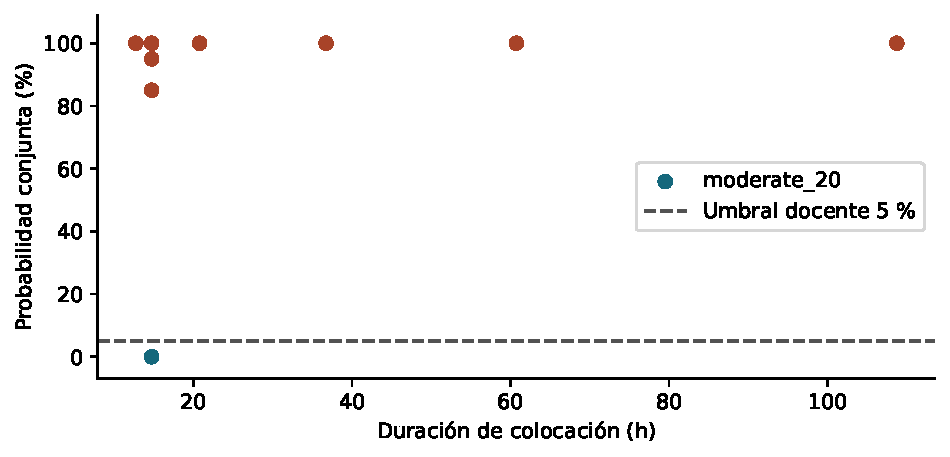
\includegraphics[width=.83\linewidth]{figuras/riesgo.pdf}
\caption{Duración y falla conjunta sobre los 24 escenarios de cada plan. Hay marcadores superpuestos en los planes de duración y riesgo coincidentes. Fuente: tabla publicada F02.}
\label{fig:risk}
\end{figure}

En F02, la envolvente $M_T=49{,}599$ °C ocurre con M4 SS, m13, a las 132,50 h en la vertida 3, en $(2{,}475;\,5{,}625;\,1{,}485)$ m. La envolvente $M_\Delta=19{,}158$ °C se obtiene con M4 SS, m17, a las 214,25 h. Concurren 47,317 °C en la vertida 3, en $(-2{,}475;\,5{,}625;\,1{,}595)$ m, y 28,159 °C junto a la base de la vertida 1, en $(-8{,}775;\,-3{,}825;\,0{,}025)$ m. En \plan{curado\_frio5} el diferencial gobernante es de M4 SS, m00, a las 642,25 h, 42,25 h después del retiro, entre un máximo interior y una superficie lateral. Estas posiciones evidencian cambios en el momento y en la frontera que gobiernan según el tipo de control. Las coordenadas son locales al IFC.

La Figura~\ref{fig:hist} toma el caso M4 SS, m17, crítico por diferencial en F02. Las curvas son extremos móviles del dominio activo y de S25 en cada instante. A diferencia de un termómetro fijo, su ubicación puede cambiar en cada estado. Las Figuras~\ref{fig:fields} y~\ref{fig:3d} muestran cortes y una vista tridimensional del campo almacenado a las 214,25 h. Aun en el programa refrigerado, el núcleo cálido se extiende a la parte gruesa y la periferia se acerca más al reservorio de suelo y al ambiente. La evidencia de campo completo publicada es representativa de un escenario, mientras que los máximos de la tabla usan la totalidad de resultados escalares. No se promedian campos para decidir cumplimiento.

\begin{figure}[htbp]
\centering
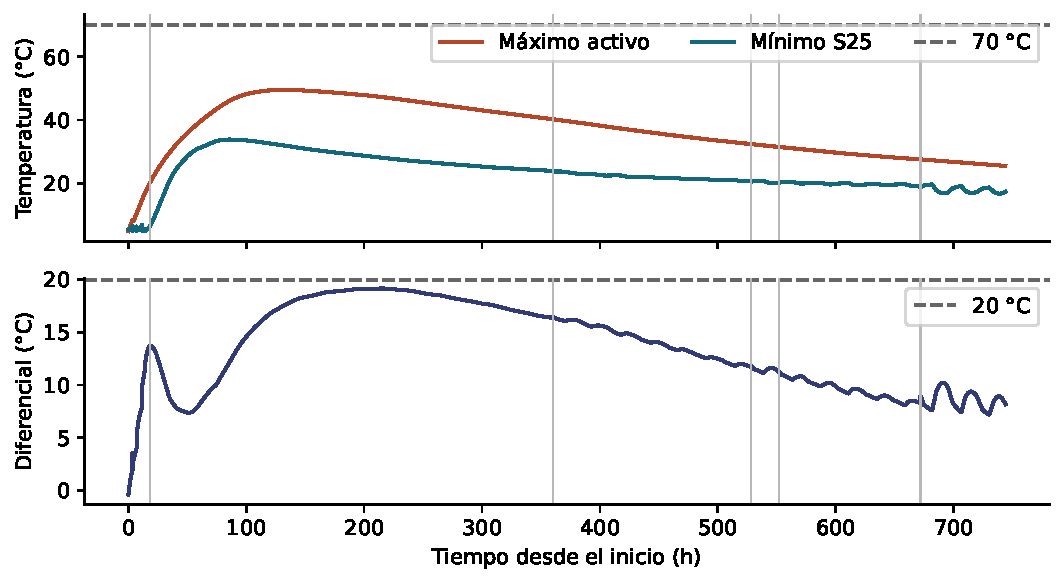
\includegraphics[width=.88\linewidth]{figuras/historia.pdf}
\caption{Extremos instantáneos del hormigón activo y de S25 para \plan{moderate\_20}, M4 SS, m17. Líneas verticales en encendido del agua, reducciones de aislación, apagado y retiro.}
\label{fig:hist}
\end{figure}

\begin{figure}[htbp]
\centering
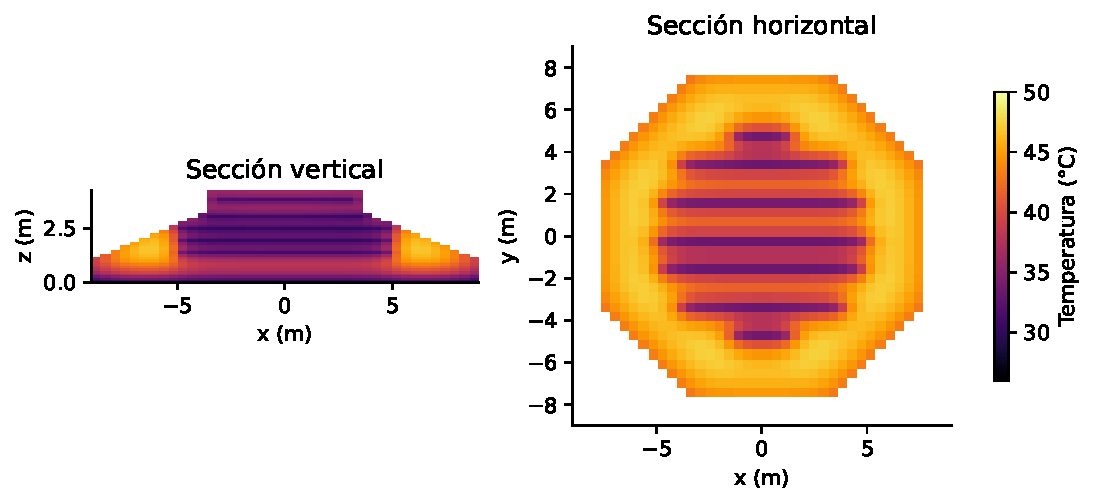
\includegraphics[width=.94\linewidth]{figuras/cortes.pdf}
\caption{Cortes del campo de temperatura a 214,25 h, vertical cerca de $y=0$ y horizontal cerca de $z=1{,}595$ m. El color comparte escala. Sólo se dibujan las celdas de hormigón. Archivo F02 \plan{fields.npz}.}
\label{fig:fields}
\end{figure}

\begin{figure}[htbp]
\centering
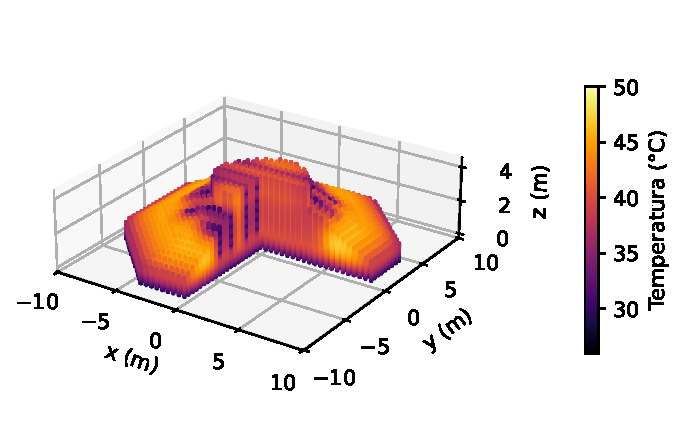
\includegraphics[width=.73\linewidth]{figuras/campo_3d.pdf}
\caption{Campo tridimensional de M4 SS, m17, a 214,25 h. Se retira un cuadrante de la representación para mostrar el interior. Cada punto es un centro de celda del archivo F02.}
\label{fig:3d}
\end{figure}

En el muestreo E14, \plan{curado\_rapido} estimó 94,49\% con intervalo de 94,025--94,929\% y \plan{curado\_frio5} estimó 84,60\% con 83,878--85,302\%. Que 95\% exacto quede fuera del primer intervalo es compatible con cobertura del 95\% a lo largo de muestras repetidas. Las seis variantes restantes tuvieron 100\% con intervalo de 99,963--100\%. La Figura~\ref{fig:mc} presenta los prefijos del banco, con su incertidumbre de muestreo. El suplemento \plan{extremos\_por\_plan.csv} registra los dos escenarios gobernantes, sus instantes y coordenadas para cada alternativa. La elección de plan usa la enumeración. Los contrastes espaciales y temporales de la Tabla~\ref{tab:control} son un segundo eje de sensibilidad, independiente de los intervalos de muestreo.
\begin{figure}[htbp]
\centering
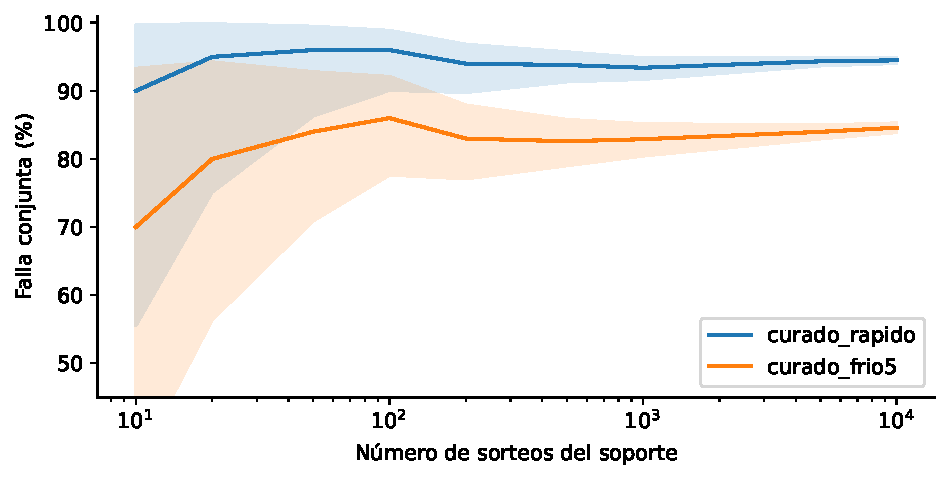
\includegraphics[width=.81\linewidth]{figuras/monte_carlo.pdf}
\caption{Trayectorias de muestreo de los dos planes pasivos de menor riesgo. Franjas de Clopper--Pearson al 95\% por cada tamaño, sin cobertura simultánea. Banco oficial E14.}
\label{fig:mc}
\end{figure}
\FloatBarrier

\section{Discusión y plan de control resultante}
El contraste con los planes pasivos ayuda a explicar dónde actuar. Una sola vertida pierde la posibilidad de dosificar en tiempo la generación de calor y concentra su pico en una masa continua. Al escalonar, una capa fría puede bajar el mínimo simultáneo mientras el material antiguo sigue generando. Las separaciones más largas de la familia protegida no redujeron lo suficiente el diferencial. En \plan{curado\_frio5}, el máximo diferencial se desplazó al período posterior al retiro. En \plan{moderate\_20}, la extracción interna reduce la energía disponible en la fase de mayor generación y el aislamiento escalonado suaviza la exposición posterior. La comparación modifica simultáneamente la refrigeración y el calendario de aislación. La diferencia observada es el efecto del paquete bajo el modelo. Estimar la contribución aislada de cada variable exigiría una comparación factorial con la otra variable fija.

Los cuatro SS dominan la cola térmica con pesos altos y energías integradas superiores. Algunas curvas 22A tienen picos de potencia incluso mayores, pero decaen antes e integran menos calor. Eso explica por qué el máximo puntual de fuente resulta insuficiente para ordenar el riesgo en una masa de baja difusividad. El clima influye tanto por la amplitud como por el instante en que coinciden enfriamiento superficial y calor retenido. El patrón pronosticado, la condición equivalente del suelo y el aislamiento desempeñan papeles diferentes en el máximo de núcleo y en el mínimo a 25 mm. Una prueba prioritaria es comprobar cómo cambian esos dos componentes cuando se usa temperatura medida del subrasante, humedades y vientos registrados y se ajusta la profundidad física del sensor. Una mezcla real diferente podría desplazar tanto la potencia como la edad del pico respecto de las curvas invertidas.

Los parámetros de diseño fijados tampoco incluyen incertidumbre por caudal desequilibrado, temperatura de retorno, pérdida de energía en conexiones, fallas de bombas, disponibilidad de agua, ciclos de parada o propiedades térmicas reales del aislante. La cercanía del diferencial refinado al límite justifica ensayar fallas y desviaciones plausibles del sistema completo antes de iniciar. Una desviación pequeña puede elevar la probabilidad ponderada por encima de 5\% si ocurre en una combinación de peso alto. La resistencia local usada en la tubería depende del tamaño de celda, por lo que el control espacial examina conjuntamente resolución de conducción, geometría de borde y representación del intercambio. Aislar estas contribuciones requeriría un contraste adicional de tubo con solución radial de referencia o una malla local independiente. También debe examinarse la resistencia de juntas y la madurez del suministro frío.

\subsection*{Plan operativo propuesto, sujeto a aprobación}
La simulación fija cinco vertidas a 5 °C, una tasa de 50 m³/h, cuatro transiciones de 30 min y el horario de la Tabla~\ref{tab:cron}. Usa ramales activos entre h 18 y 552 con agua de entrada a 20 °C y las tres etapas de retiro. Esas son las condiciones simuladas que definen la recomendación probabilística. Las acciones siguientes trasladan la propuesta a un protocolo revisable y requieren aprobación del proyectista y de la inspección técnica.

\begin{enumerate}
\item \textbf{Antes del inicio.} El jefe de obra coordina el calendario, los relevos y el suministro frío con la planta. La inspección verifica la geometría y las cotas; el proyectista revisa juntas, compatibilidad con armaduras, pasadas, colectores, estanqueidad y disposición final de circuitos. El especialista hidráulico realiza prueba de presión y medición de caudales, confirma redundancia y revisa capacidad frigorífica a plena operación. Se contrasta con una prueba piloto y se acuerdan tolerancias respecto de los 5 °C especificados.
\item \textbf{Durante la colocación.} El responsable de calidad registra temperatura y hora de cada camión o carga al recibir y al descargar, caudal efectivo de colocación e inicio y fin de cada etapa. La inspección contrasta esos valores con el cronograma y decide antes de la siguiente etapa si se mantiene, reprograma o interrumpe la secuencia. Se usan sondas duplicadas en el núcleo de V3, con puntos cerca de las posiciones cálidas de la sección anterior, en la base de V1 y junto al lateral susceptible de gobernar. Se incluyen sondas cerca y lejos de un tubo para detectar enfriamiento localizado.
\item \textbf{Protección y curado.} Las sondas superficiales se disponen a 25 mm medidos desde la cara real, con especial atención a la cota cero y a laterales próximos al contorno IFC. Se instala una estación ambiente protegida y se registra temperatura y caudal de entrada y retorno por colector, además del estado de ramales y bombas. Una adquisición propuesta es cada 5 min con registro horario revisado por el supervisor térmico y alarmas continuas. El diferencial operativo se calcula simultáneamente sobre los sensores funcionales. Su capacidad para acotar los extremos se verifica con redundancia y comparación con el campo previsto.
\item \textbf{Alertas y medidas.} Como umbrales preventivos propuestos se revisa el protocolo al alcanzar 65 °C en el núcleo o 18 °C de diferencial y al observar una tendencia que los alcance antes de la siguiente revisión. Con falla de caudal, fuga, pérdida de sondas o temperatura fuera de rango se mantiene la protección y se activa el equipo de respaldo o se aísla el circuito afectado según el diseño aprobado. Se comprueba que el ajuste de agua no enfríe bruscamente ninguna zona. Si se alcanzan 70 °C o 20 °C, se conserva el historial, se escala al proyectista y se bloquea el retiro hasta resolver el desvío. La inspección documenta la causa, las medidas y la autorización para continuar.
\item \textbf{Retiro y cierre.} El supervisor comprueba las tendencias de núcleo y superficies antes de cada reducción de espesor. Ante un pronóstico de enfriamiento abrupto o aumento del diferencial se posterga el retiro o se mantiene protección adicional previa evaluación. Se vigila por lo menos durante la ventana de 72 h posterior al retiro simulado, con extensión si las mediciones lo requieren. La liberación estructural depende de criterios adicionales de resistencia y madurez.
\end{enumerate}
El piloto y la primera aplicación instrumentada permitirían cotejar energía extraída, temperaturas locales y gradientes con predicciones registradas con antelación. La comparación debería reservar observaciones independientes para validación y declarar cuáles se destinaron a calibrar. También permitiría acordar márgenes de acción medibles, pues un sensor mal colocado o una tolerancia instrumental comparable con 0,379 °C afecta la decisión. La operación monitorizada y sus contingencias se proponen para implementación. No tienen un riesgo ya cuantificado en el soporte de 24 escenarios.

\section{Conclusiones}
Entre los nueve programas, \plan{moderate\_20} es el único que satisface el límite de falla en el modelo nominal y por ello el más rápido entre los factibles. Termina la colocación a las 14,738 h, con cinco etapas, menor temperatura inicial, tuberías con agua y protección escalonada. La vertida única termina en 12,738 h y registra 100\% de falla; el programa con pausas de 6 h emplea 36,738 h y registra 100\%. El mejor plan anterior en probabilidad registra 85\% a la misma duración de colocación del programa refrigerado. En las 744 h de \plan{moderate\_20}, los máximos nominales son 49,599 °C y 19,158 °C y la probabilidad conjunta ponderada es 0\%, con cero excedencias en los 24 casos. El control espacial más exigente arroja 19,621 °C.

La recomendación se circunscribe a los planes y escenarios estudiados. El margen espacial observado, la localización de S25 y la evidencia parcial de refinamiento son las limitaciones inmediatas para certificar el cumplimiento. Antes de aplicar el plan corresponde validar el trazado y la hidráulica, confirmar la temperatura y capacidad del suministro, comprobar juntas y aislación, y contrastar la respuesta con una prueba instrumentada. El mismo conjunto de ensayos debe incluir desviaciones plausibles de clima, material y operación y avanzar hacia una evaluación numérica más completa. Con esa evidencia podrá revisarse la decisión y su incertidumbre, separando siempre el criterio térmico docente del riesgo mecánico de fisuración.

\begin{thebibliography}{9}
\bibitem{aci} ACI Committee 207. \emph{Guide to Mass Concrete}. ACI 207.1R-05, American Concrete Institute, 2005.
\bibitem{ciria} P. B. Bamforth. \emph{Control of cracking caused by restrained deformation in concrete}. CIRIA C766, Londres, 2018.
\bibitem{gnielinski} V. Gnielinski. New equations for heat and mass transfer in turbulent pipe and channel flow. \emph{International Chemical Engineering}, 16(2), 359--368, 1976.
\bibitem{cp} C. J. Clopper y E. S. Pearson. The Use of Confidence or Fiducial Limits Illustrated in the Case of the Binomial. \emph{Biometrika}, 26(4), 404--413, 1934. \href{https://doi.org/10.1093/biomet/26.4.404}{doi:10.1093/biomet/26.4.404}.
\bibitem{openmeteo} Open-Meteo. \emph{Ensemble Weather API}. Documentación del producto. \url{https://open-meteo.com/en/docs/ensemble-api}. Instantánea usada identificada en el Anexo~\ref{app:repro}.
\bibitem{e14} Grupo 2, MCOC. \emph{Proyecto 2, E14: Monte Carlo, incertidumbre y ejecución paralela}. Incluye referencia docente en \plan{data/references/criterio\_curso.json}. \href{https://github.com/amvaras/Proyecto-2-MCOC/tree/f9d2faa150f9fdda007679386568326497f0d239/P2_E14}{Repositorio, versión E14}.
\bibitem{e15} Grupo 2, MCOC. \emph{Entrega E15: Comparación probabilística de planes}. \href{https://github.com/amvaras/Proyecto-2-MCOC/blob/0bb141827d24f7bed24137fad86119998f10e743/P2_E15/Entrega_E15_MCOC.md}{Repositorio, versión E15}.
\bibitem{f02} Grupo 2, MCOC. \emph{Evidencia F02: Enfriamiento interno, campos y controles}. \href{https://github.com/amvaras/Proyecto-2-MCOC/tree/969c8141f3daf4b9e6c7778f29bfe34d937e9fe5/P2_E14}{Repositorio, exportación de defensa}.
\end{thebibliography}
\clearpage
\appendix
\section{Trazabilidad y reproducción}\label{app:repro}
El archivo \plan{REPRODUCCION.md}, junto al fuente editable, contiene comandos para compilar el artículo, regenerar gráficas, recuperar los resultados de la defensa, verificar E14 y volver a simular con F02. Las versiones de referencia son las siguientes.
\begin{center}\small
\begin{tabular}{@{}ll@{}}
\toprule
Componente & SHA-1 de Git \\
\midrule
Exportación de defensa & \texttt{969c8141f3daf4b9e6c7778f29bfe34d937e9fe5} \\
E14 & \texttt{f9d2faa150f9fdda007679386568326497f0d239} \\
E15 & \texttt{0bb141827d24f7bed24137fad86119998f10e743} \\
\bottomrule
\end{tabular}
\end{center}
Las entradas, el solver y sus resultados se conservan. F01 recompone gráficos y análisis descriptivo a partir de esa evidencia, incluidos cálculos de sensibilidad algebraica.

El suplemento \nolinkurl{riesgo_336h_e14.csv} reproduce la agregación comparativa en el intervalo común. El archivo \plan{escenarios\_f02.csv} contiene las 24 filas de \plan{moderate\_20} con curva, clima, peso, métricas, indicadores, tiempos y coordenadas. Los ocho planes anteriores conservan su índice de 192 filas en \plan{results/e14/official.json}. Los configuradores son \plan{configs/e14/study.json} y \plan{configs/f02/moderate\_20.json}. Los insumos son \nolinkurl{geometry/foundation.ifc}, \nolinkurl{data/hydration/source_terms.txt} y \nolinkurl{data/ensemble/}, con historias horarias en \plan{data/weather/}. El SHA-256 del pronóstico sin procesar archivado se identifica en \plan{data/ensemble/metadata.json}. La masa de probabilidad es $0{,}20$ por cada SS y $0{,}05$ por cada 22A, multiplicada por las frecuencias $15/31$, $12/31$ o $4/31$ según el medoide.

\section{Constancias para revisión académica}
La autoría figura como Grupo 2 hasta confirmar la nómina y el orden de firmas. La fecha de portada identifica la preparación del artículo. El encargo reproduce el vencimiento como «viernes 23 de noviembre de 2026». El 23 de noviembre de 2026 corresponde a lunes y la fecha y hora definitivas se deben confirmar en Canvas. Está pendiente constancia de aprobación del Centro de Escritura. La auditoría que acompaña al artículo coteja los siete criterios de F01 e informa una estimación de revisión sobre 10 puntos.
\end{document}
